\subsection{Open loop simulation of passive components}

To check that the calculations have been made correctly, an open loop simulation of the circuit with only passive components was done. As it can be seen in figure \ref{openloop} the circuit consists of the 4 MOSFETs, the inductor, the 2 capacitors and a load. The MOSFETs is controlled with two dutycycles D1 and D2. FET1 and FET2 will get the actual dutycycle that are used while FET3 and FET4 uses NOT operators to get the opposite values of FET1 and FET2. With the scope the output voltage and current through the inductor can be seen.

\begin{figure}[H]
	\begin{center}
		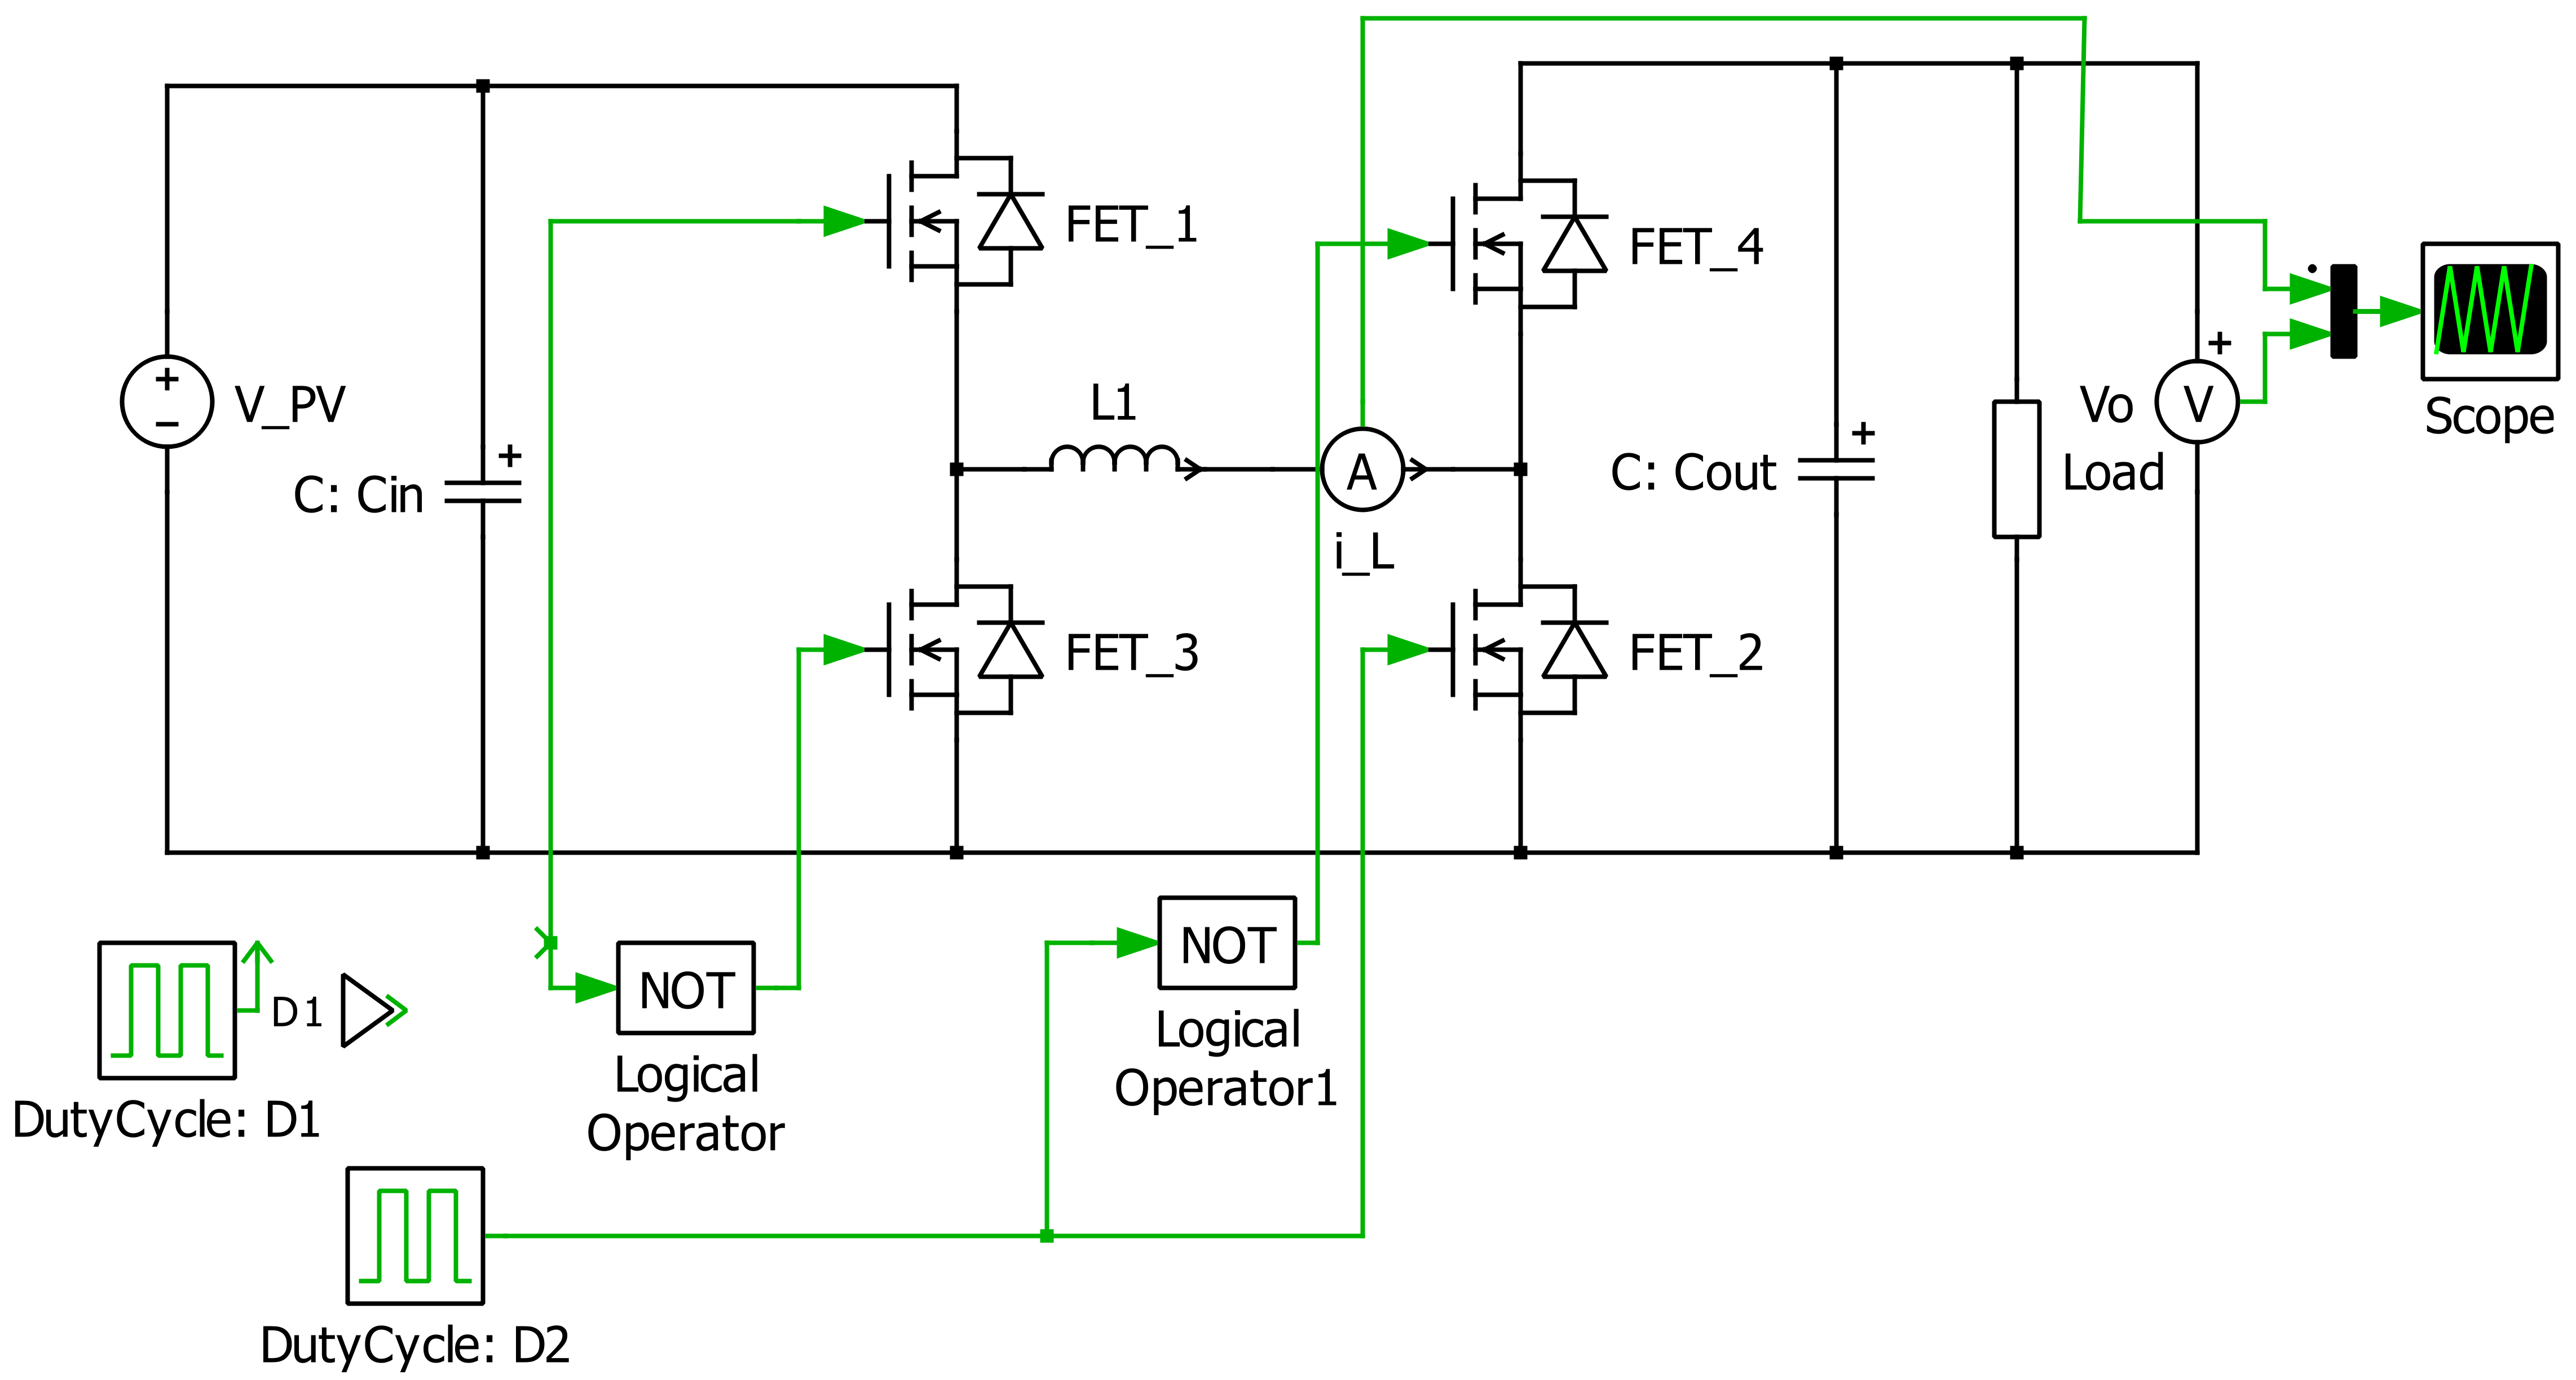
\includegraphics[width=0.7\textwidth]{../Pictures/openloop}
		\caption{Ideal open loop simulation}
		\label{openloop}
	\end{center}
\end{figure}
\todo{Modify this figure because the duty cycle D1 is not connected. Stef}
The values for the components are $C_{in}=1880\mu F$, $C_{out}=820\mu F$ and $L1=1mH$ as described earlier and $V_{in}=32.6V$. At first the buck mode is simulated. In this mode D2 is 0. This means that FET2 is 0 and FET4 is one because of the NOT operator. The dutycycle for D1 and thereby FET1 is sat to 0.736 which was calculated in \ref{buckduty}. This should give an output voltage of 24V which can be seen in figure \ref{bucksimulation}. The load is $1.92\Omega$ because that gives 300W with an output voltage of 24V.     
\begin{figure}[H]
 	\begin{center}
 		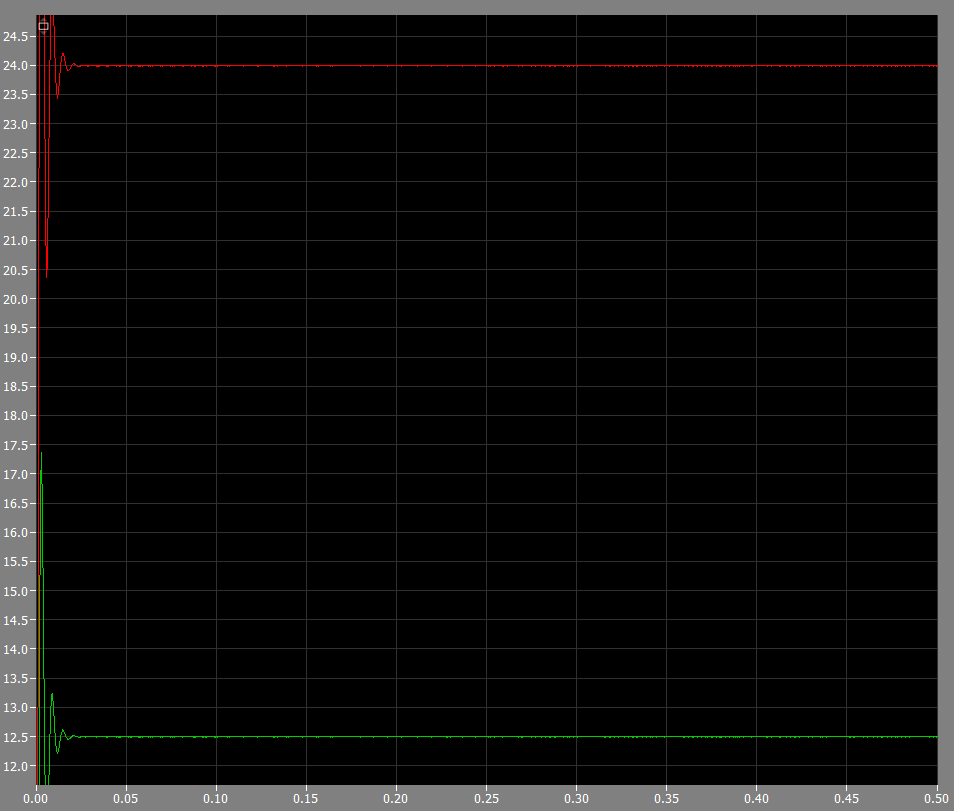
\includegraphics[width=0.5\textwidth]{../Pictures/bucksimulation24}
 		\caption{open loop simulation of buck mode}
 		\label{bucksimulation}
 	\end{center}
\end{figure} 
\todo{Modify this scope!In PLECS there is an option to export the scope and it will have a white background. Also make the figure bigger and the line width of the signals is hard to see. I use for the simulation results graphs a linewidth of 1.1. Stef}
In buck mode the current through the inductor should be equal to the output current \ref{iavg} which with a load of $1.92\Omega$ should be:
\begin{equation}
I_{out} = \frac{V_{out}}{\Omega} = \frac{24V}{1.92\Omega} = 12.5A
\end{equation}   

To test the boost mode the input voltage is the same. Here the dutycycle for D2 is 0.638. This is for an output voltage of 90V and calculated with the same equation as \ref{boostD}. D1 is sat to 1 so that FET1 is one and FET3 is 0 because of the NOT operator. This should give and output voltage of 90V. With 90V the output current should be 9A and then the current through the inductor is calculated like this:

\begin{equation}
I_{L} = \frac{1}{1-0.638}\cdot 12.5A = 9.207A
\end{equation}  

In figure \ref{boostsim} steady state the red line is again the output voltage which is the expected 90V just as the green line which is the current through the inductor is a bit more than 9A.

\begin{figure}[H]
	\begin{center}
		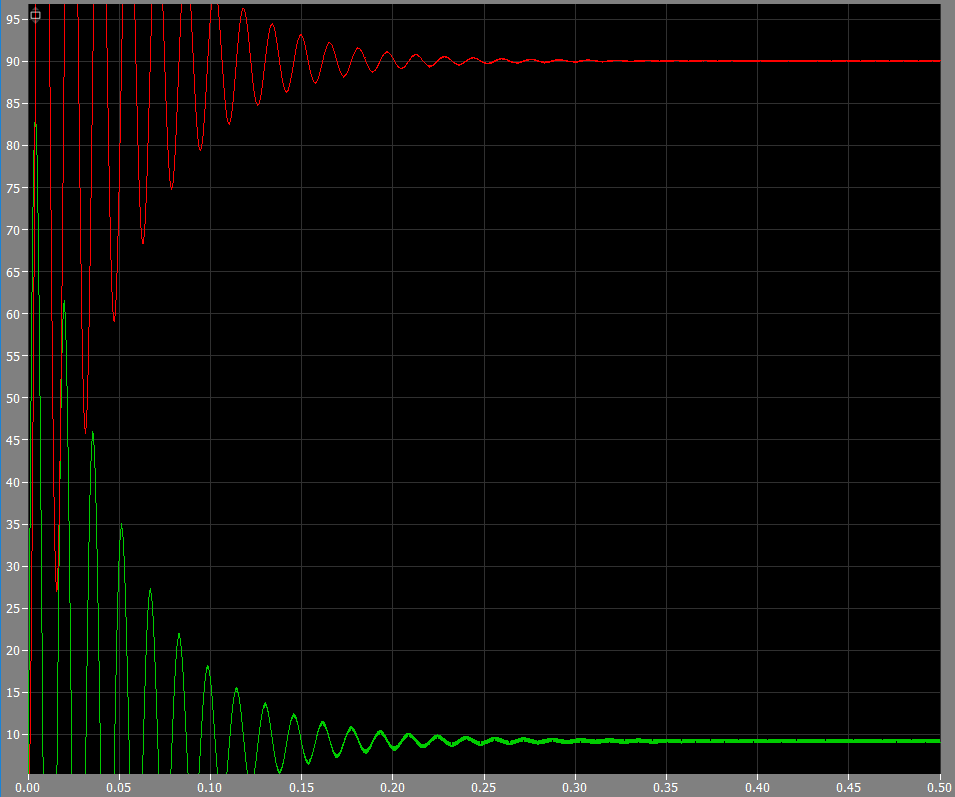
\includegraphics[width=0.5\textwidth]{../Pictures/boostsim}
		\caption{open loop simulation of boost mode}
		\label{boostsim}
	\end{center}
\end{figure}
